\section{Appendix}\label{appendix}
The appendix contains two figures as presented in the indicated sources, showcasing results of the respective approaches.
\begin{figure}[htbp]
 \centering
 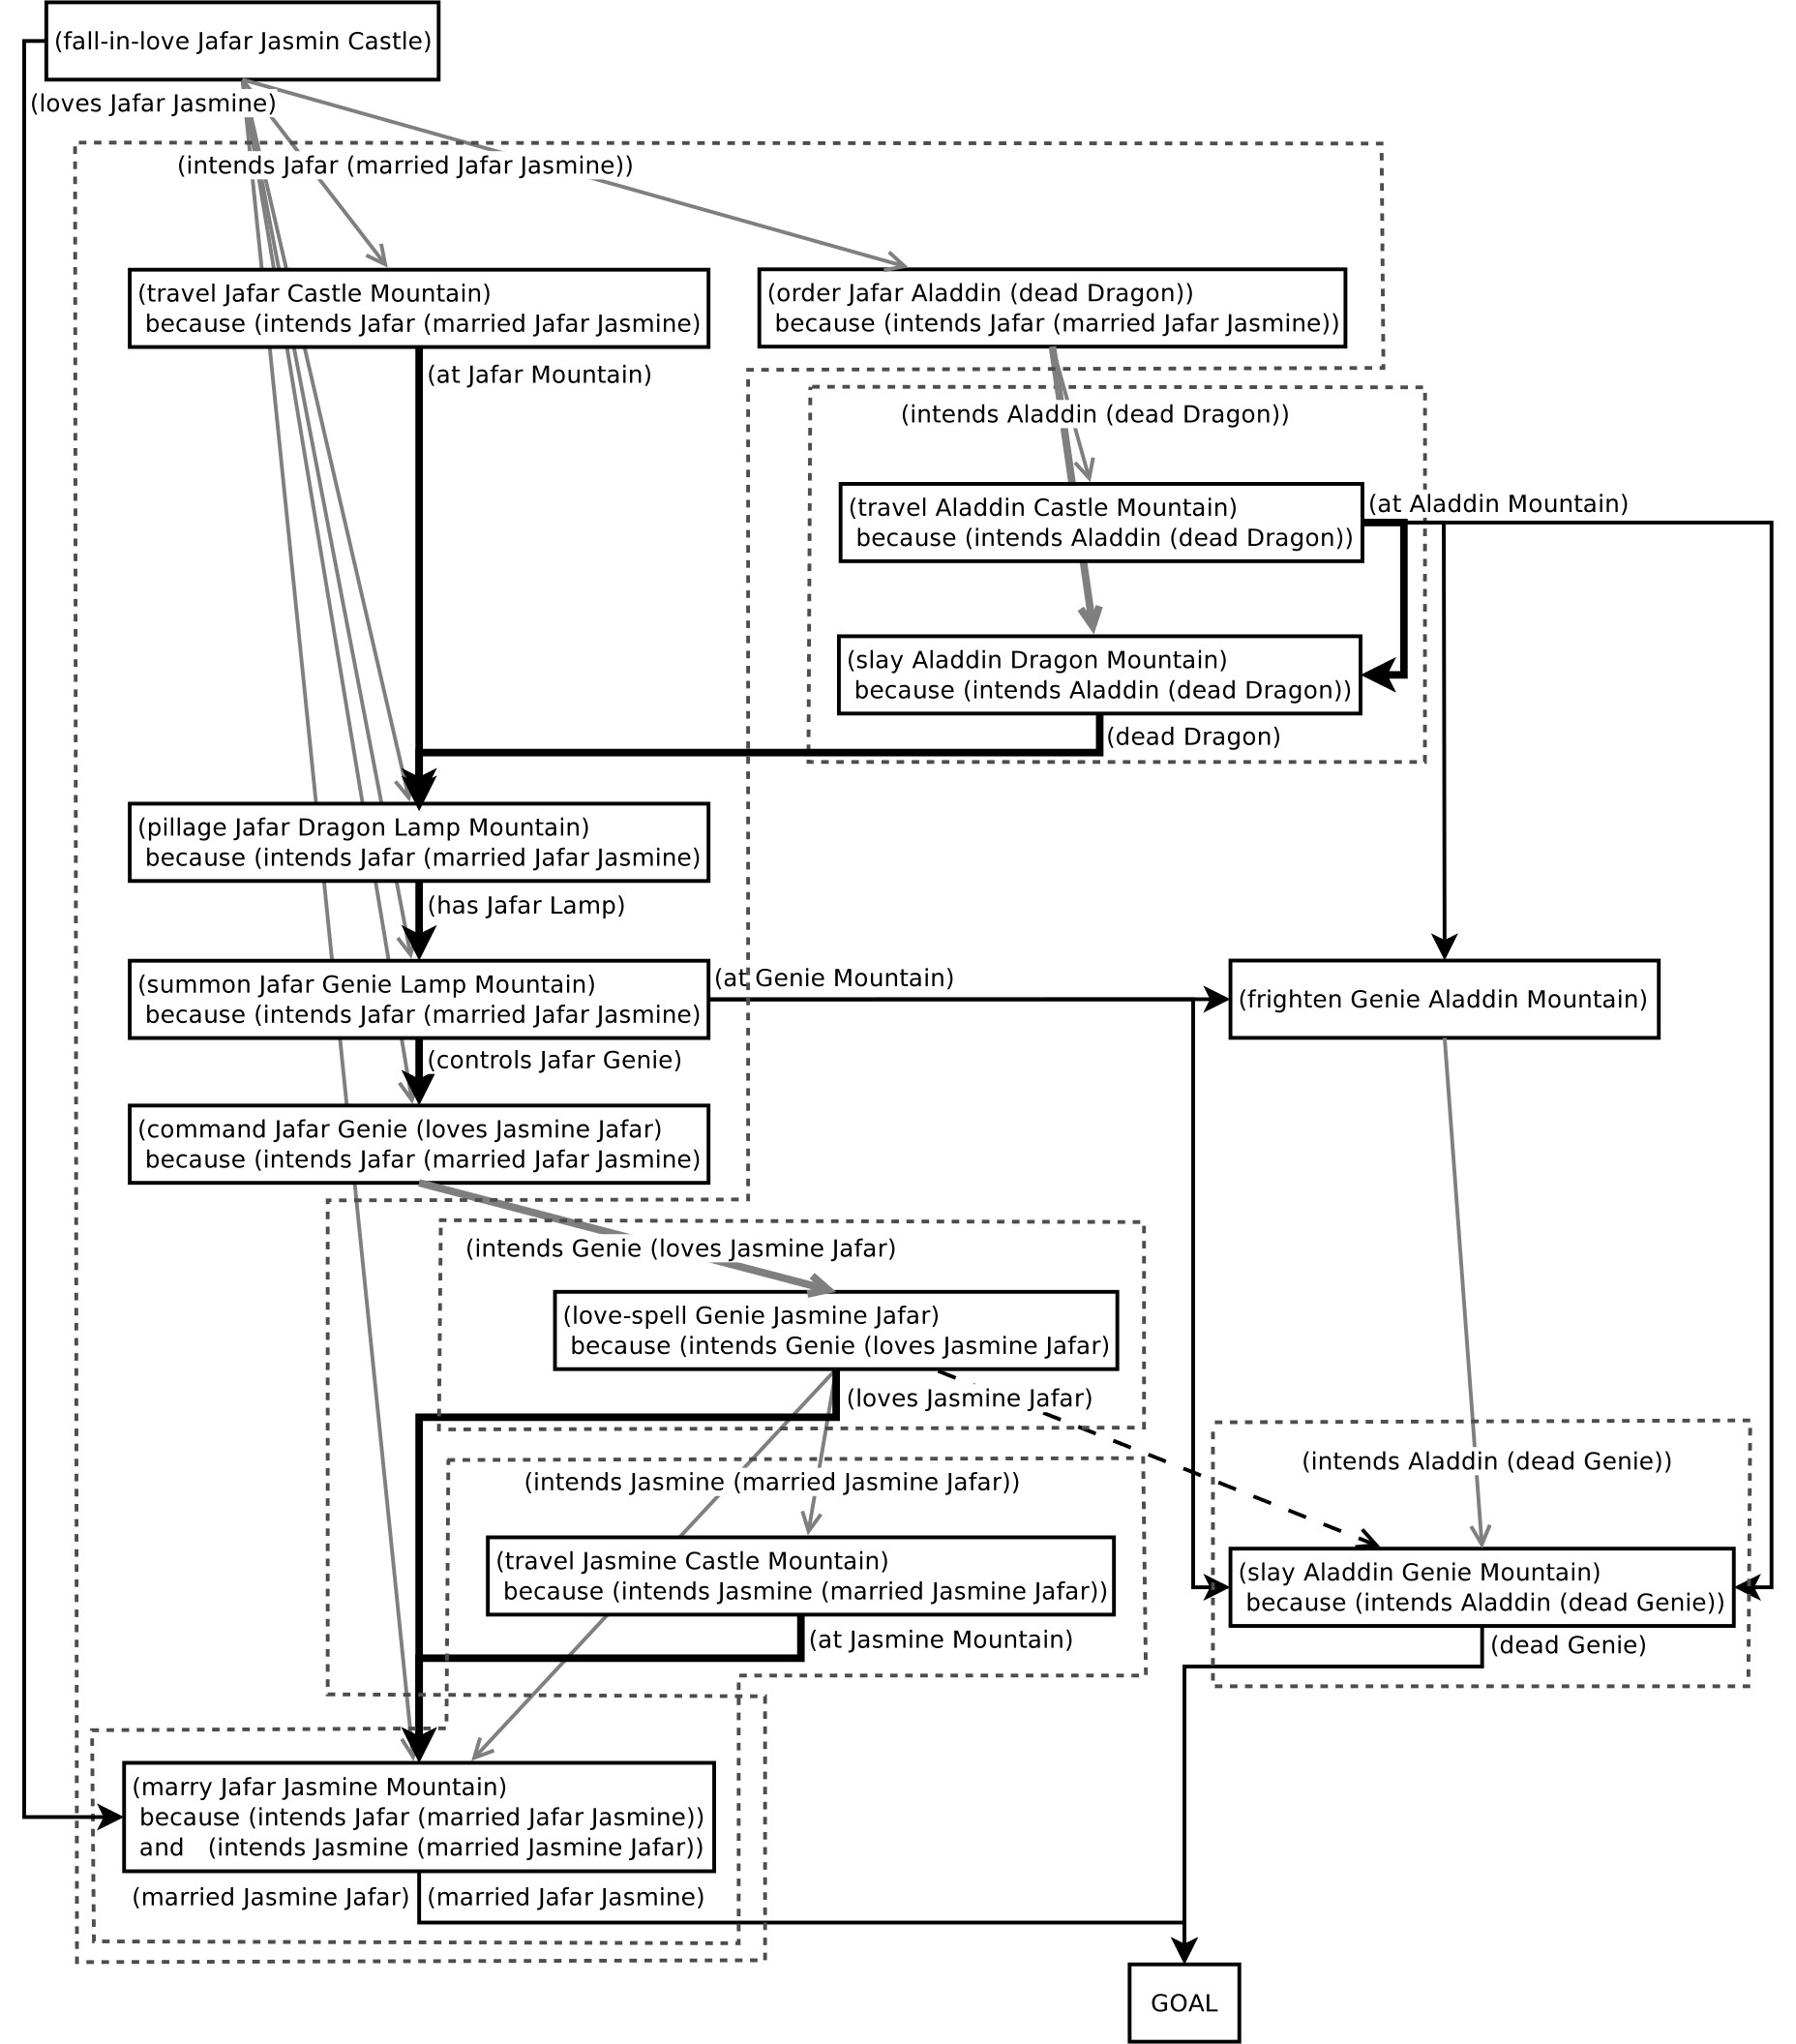
\includegraphics[scale=0.2]{haslum_result}
 \caption{''A story plan generated for the example problem. Motivational links are drawn in gray. The dashed edge is an ordering constraint. The outlines group actions that form a frame of commitment for a character. To avoid clutter, causal links for justified predicates are not shown; instead, causal links from the chosen effect of each action are drawn in bold. It can be seen that each chosen effect, except for final steps, links (directly or indirectly) to a precondition of an action in the same frame of commitment.'' \cite{Haslum14}}
 \label{fig:a1}
\end{figure}
\begin{figure}[htbp]
 \centering
 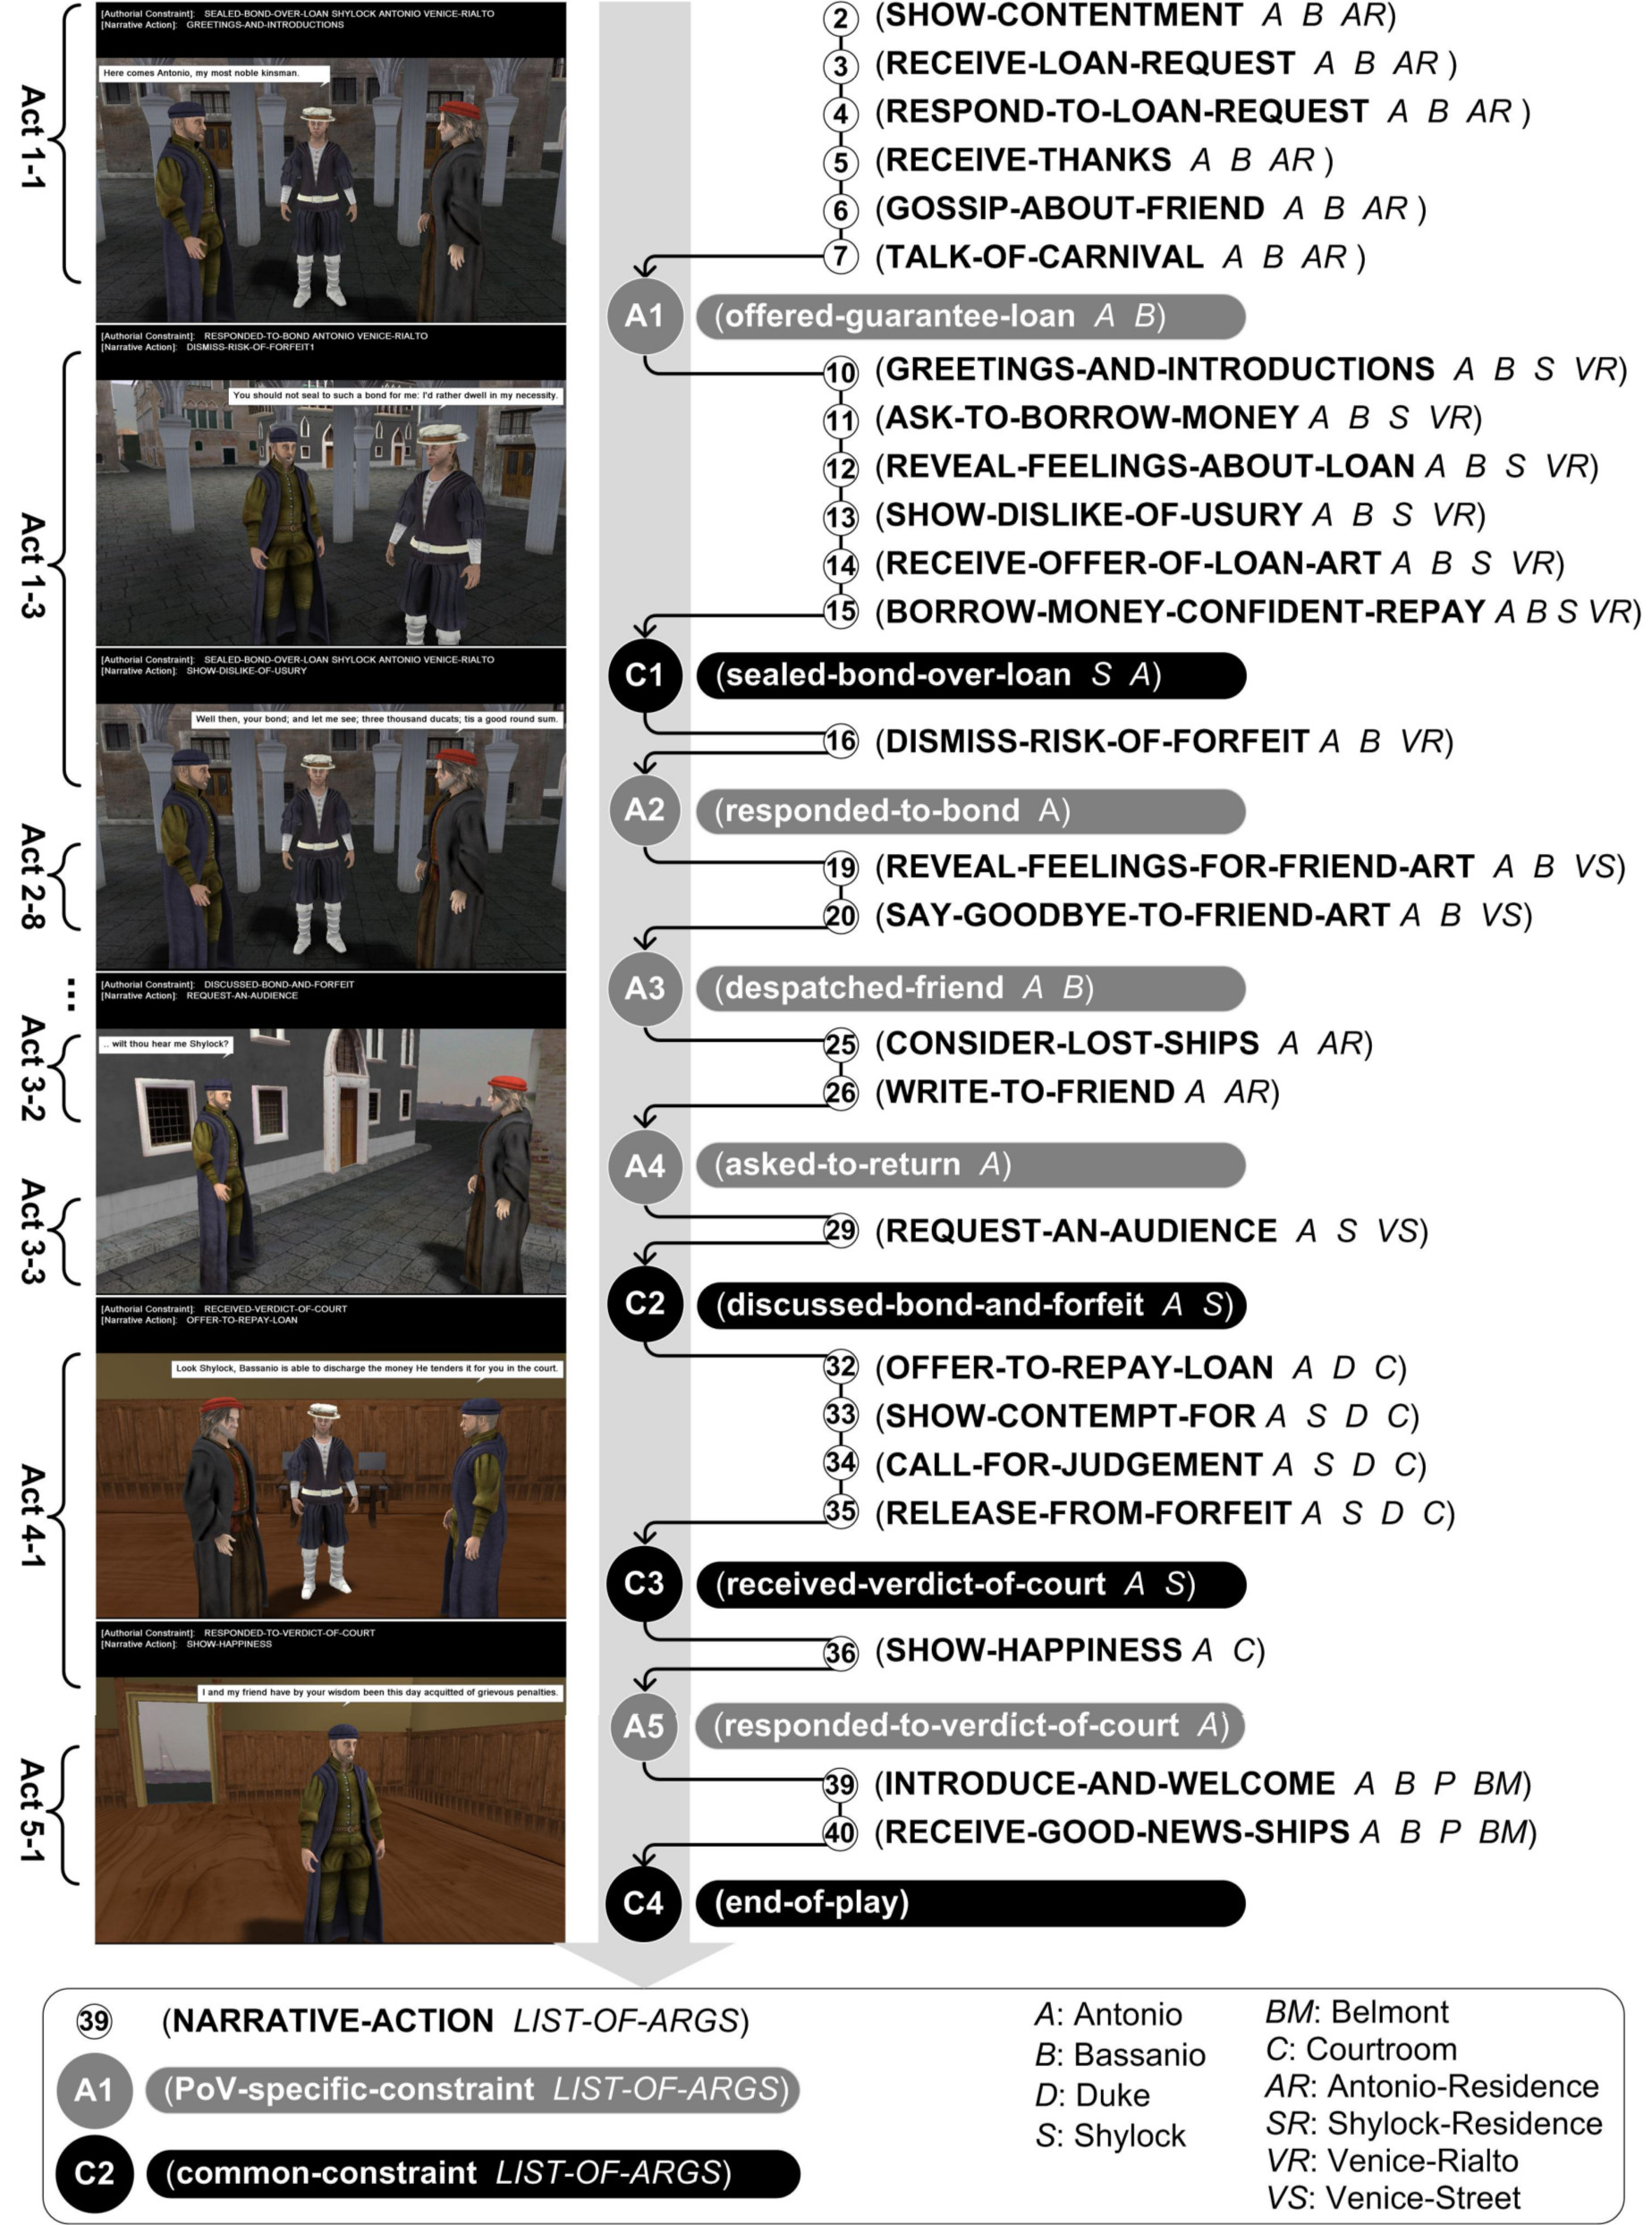
\includegraphics[scale=0.2]{porteous_result}
 \caption{''A single generated narrative for the pound-of-flesh sub-plot with (pov antonio-risk-taker). Key constraints selected by the generator are highlighted (A1, C1, A2, A3, A4, C2, C3, A5, C4) and are preceded by the sequences of narrative actions selected to achieve them. This variant shows a carefree Antonio who confidently borrows money and continually dismisses personal risks even when brought to trial for defaulting on the loan. It ends with Antonio celebrating his release.'' \cite{Porteous10}}
 \label{fig:a2}
\end{figure}
